\documentclass[a4paper,11pt]{report}

\usepackage{fullpage}

\usepackage{amsmath}
\usepackage{bussproofs}
\usepackage{mathpartir}
\usepackage{prooftrees}
\usepackage{color}
\usepackage{hyperref}
\usepackage{placeins}


% for finite state automata
\usepackage{tikz}
\usetikzlibrary{automata,positioning}

%%%%%%%%%%%%%%%%%%%%%%%%%%%%%%%%%%%%%%%%%%%%%%%%%%%%%%%%%
% Minted
%%%%%%%%%%%%%%%%%%%%%%%%%%%%%%%%%%%%%%%%%%%%%%%%%%%%%%%%%

\usepackage[cache=false]{minted}

\newmintinline{c}{
  fontsize=\small,
  breaklines=true
}

\newminted{c}{
  frame=single,
  framesep=2mm,
  fontsize=\scriptsize,
  mathescape
}

\newminted[ccodeline]{c}{
  frame=single,
  framesep=2mm,
  fontsize=\scriptsize,
  mathescape,
  linenos
}

% End minted
%%%%%%%%%%%%%%%%%%%%%%%%%%%%%%%%%%%%%%%%%%%%%%%%%%%%%%%%%


\author{Sylvain Julmy}
\date{\today}

\setlength{\parindent}{0pt}

\begin{document}

\begin{center}
  \Large{
    Operating Systems\\
    Spring 2018
  }
  
  \noindent\makebox[\linewidth]{\rule{\linewidth}{0.4pt}}
  S02
  \noindent\makebox[\linewidth]{\rule{\linewidth}{0.4pt}}

  \begin{flushleft}
    Professor : Philippe Cudré-Mauroux

    Assistant : Ines Arous
  \end{flushleft}
  
  \noindent\makebox[\linewidth]{\rule{\linewidth}{0.4pt}}

  Submitted by Sylvain Julmy
  
  \noindent\makebox[\linewidth]{\rule{\textwidth}{1pt}}
\end{center}

\section*{Exercice 2}

For the exercice, I have choose the following commands :
\begin{itemize}
\item \verb+perf bench+
\item \verb+top+
\item \verb+kill+
\end{itemize}

\subsection*{\texttt{perf bench}}

\verb+perf bench+ is a command that can launch a set of multi-threaded
benchmarks to exercice various subsystems in the Linux kernel and system calls.

This command allow any devolopper to easely create benchmarks and run them in
Linux. It is very usefull to test some very specific instructions of the
microprocessor like \textbf{Compare-And-Swap} (CAS).

The figure~\ref{fig:perf-bench-mem} shows an example of an execution of the
command. The system perform benchmarks for memory test.

\begin{figure}[ht]
  \centering
  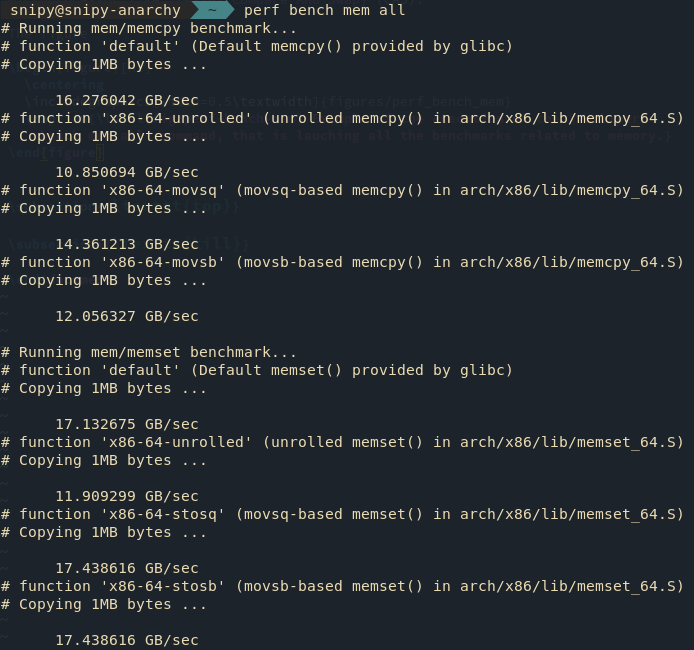
\includegraphics[width=0.8\textwidth]{figures/perf_bench_mem}
  \caption{\label{fig:perf-bench-mem} Example of the execution of the \texttt{perf
    bench mem all} command, that is lauching all the benchmarks related to memory.}
\end{figure}

\subsection*{\texttt{top}}

The \verb+top+ command provides a dynamic real-time view of a running
system. It can display system summary information as well as a
list of processes or threads currently being managed by the Linux
kernel\footnote{\url{https://perf.wiki.kernel.org/index.php/Tutorial}}.

The figure~\ref{fig:top} shows the run of the command, we can show all the
information related before (and in series 01).

\begin{figure}[ht]
  \centering
  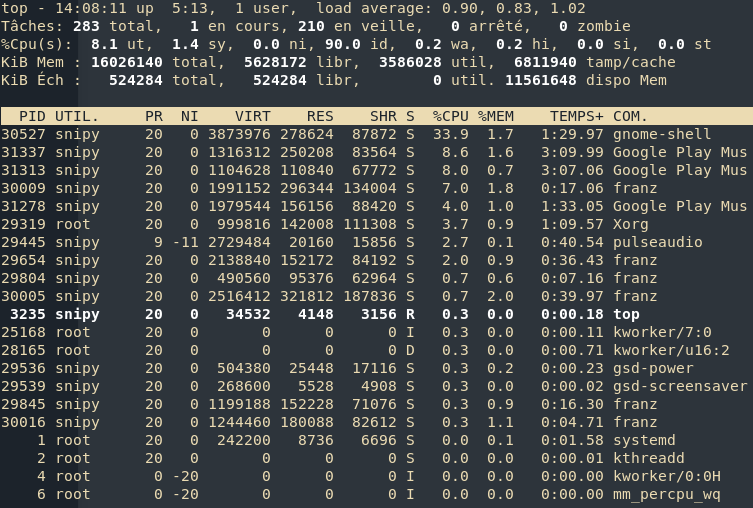
\includegraphics[width=0.8\textwidth]{figures/top}
  \caption{\label{fig:top} Execution of the \texttt{top} command, relevant
    information like Cpu usage, memory or processes are display.}
\end{figure}

\subsection*{\texttt{kill}}

The command \verb+kill+ is used to send specific signal to the specified
processes or process groups. A special case of this command is \verb+kill -9+
where the process is simply killed by the command, this signal cannot be caught
or ignored, and the receiving process cannot perform any clean-up upon receiving
this signal.

There are some exceptions\footnote{\url{https://en.wikipedia.org/wiki/Signal_(IPC)}} :
\begin{itemize}
\item Zombie processes cannot be killed since they are already dead and waiting
  for their parent processes to reap them.
\item Processes that are in the blocked state will not die until they wake up
  again.
\item The init process is special: It does not get signals that it does not want
  to handle, and thus it can ignore SIGKILL. An exception from this exception
  is while init is ptraced on Linux.
\item An uninterruptibly sleeping process may not terminate (and free its
  resources) even when sent SIGKILL. This is one of the few cases in which a
  UNIX system may have to be rebooted to solve a temporary software problem.
\end{itemize}

\FloatBarrier

\section*{Exercice 3}

\begin{ccodeline}
  int f(int x) {
    int y = 4;
    return x + y + 2;
  }
  int main(int argc, const char * argv[]) {
    int x = 4;
    f(x);
    return 0;
  }
\end{ccodeline}

\newpage

\subsection*{End of line 6}

\begin{figure}[h]
  \centering
  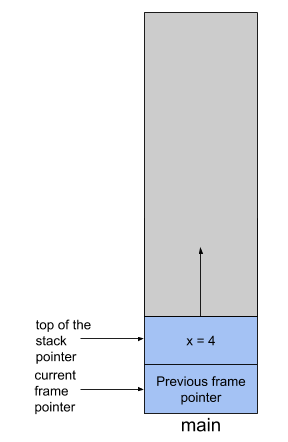
\includegraphics[width=0.3\textwidth]{figures/ex3_schema1}
\end{figure}

\FloatBarrier

\subsection*{End of line 2}

\begin{figure}[h]
  \centering
  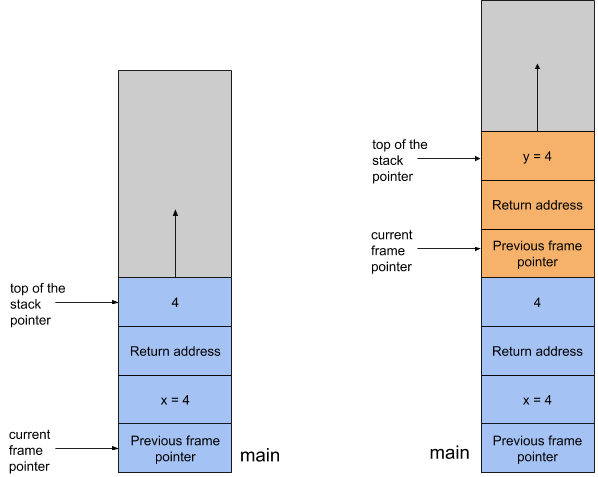
\includegraphics[width=0.6\textwidth]{figures/ex3_schema2}
\end{figure}

\FloatBarrier

\newpage

\subsection*{End of line 3}

\begin{figure}[h]
  \centering
  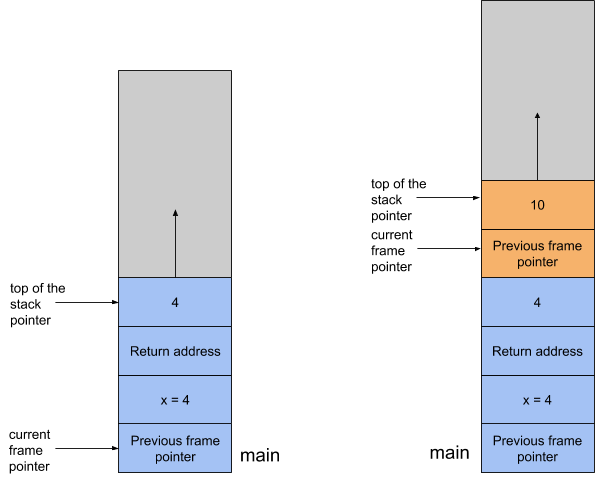
\includegraphics[width=0.6\textwidth]{figures/ex3_schema3}
\end{figure}

\FloatBarrier

\subsection*{End of line 8}

\begin{figure}[h]
  \centering
  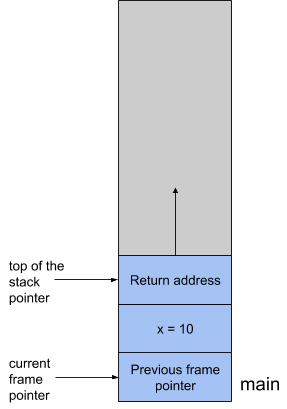
\includegraphics[width=0.3\textwidth]{figures/ex3_schema4}
\end{figure}

\FloatBarrier

\section*{Exercice 4}

\begin{table}[h]
\centering
\begin{tabular}{|l|l|l|}
\hline
\textbf{Location of referenced word} & \textbf{Probability} & \textbf{Total time for access in ns} \\ \hline
Cache                                & $0.9$                & $30$                                 \\ \hline
Not in cache but in main memory      & $0.1 * 0.7 = 0.07$   & $30 + 70 = 100$                      \\ \hline
Not in cache or in main memory       & $0.1 * 0.3 = 0.03$   & $100 + 22ms = 22'000'100$            \\ \hline
\end{tabular}
\end{table}

The average access time is :

\[
  avg = 0.9 * 20 + 0.06 * 100 + 0.04 * 22'000'100 = 880'028 ns
\]

\section*{Exercice 5}

Yes, if the stack is only used to store the return address, then the program
counter can be eliminated. In the case where the stack is also used to store the
parameters, then, at a certain point in time, the processor would need both a
parameter and the program counter on top of the stack at the same time.

\end{document}
